\section{Studiendurchführung}

Der Proband setzt sich in einen bequemen Stuhl, welcher von ihm nach Belieben verstellt werden kann. Nach kurzen Instruktionen zum Ablauf und zur Bedienung des VR-Controllers, wird dem Proband die VR-Brille aufgesetzt, woraufhin er als erstes in der virtuellen Umgebung einen SAM-Fragebogen ausfüllen muss. %sagt man dazu SAM-Fragebogen?
Bevor die eigentliche Studie beginnt, hat der Proband die Möglichkeit, sich ein wenig mit der Steuerung vertraut zu machen, indem er in der Umgebung den Controller verwendet, um schwebende Blasen platzen zu lassen, eine Mechanik die in allen drei späteren Aufgaben von elementarer Bedeutung sein wird. Sobald die Testperson durch das klicken auf einen Button angibt, bereit zu sein, beginnt die Schlafphase. Diese beträgt bei jedem einzelnen Probanden exakt 15 Minuten, jedoch wurde ihnen vor der Studie mitgeteilt, dass die Dauer zwischen 15 und 25 Minuten variiere. %Zeit nochmal checken
Bei unseren ersten 30 Teilnehmern wurde ein heller Lichtreiz verwendet um die Probanden aus dem Schlaf beziehungsweise aus ihrer Entspannung zu reißen. Bei 15 von ihnen dauerte es 20 Sekunden bis der Lichtreiz seine volle Helligkeit erreichte, wohingegen bei der anderen Hälfte der Lichtreiz fünf Sekunden benötigte um sich vollkommen zu entfalten.  Die restlichen 15 Probanden wurden nicht visuell, sondern durch das Geräusch einer Autoalarmanlage geweckt. %Zeiten checken!
Jeder Proband wurde innerhalb dieser Phase beobachtet, damit neben Informationen zum Stuhl (Winkel der Lehne) auch festgehalten werden konnte, wie unruhig beziehungsweise entspannt jeder einzelne von ihnen war. Ferner wurde jeder nach zehn Minuten nochmal genauer inspiziert, hierbei wurde die Atmung des Versuchsteilnehmers analysiert.
Bei allen 45 Testpersonen folgte nach dem Wecken die exakt identische Prozedur. Zunächst mussten sie auf einen Startbutton drücken um mit den Aufgaben zu beginnen. Die im Abschnitt 'Aufgaben' geschilderten Tasks wurden stets in derselben Reihenfolge von den Probanden abverlangt. Zuerst das Zahlen sortieren, gefolgt vom Farbspiel und zuletzt das zählen der Blöcke. %Noch überlegen, wie wir diese Spiele wirklich nennen wollen.
Sobald der Proband alle drei Aufgaben absolviert hat, muss er abermals den gleichen SAM-Fragebogen wie zuvor ausfüllen und darüber hinaus noch zusätzlich auf die Frage antworten, als wie anspruchsvoll er die gestellten Aufgaben erachtete.
Schlussendlich darf die VR-Brille abgesetzt werden, woraufhin der Proband als letztes noch an einer demographischen Umfrage, welche diesmal nicht in VR stattfindet, sondern an einem Computer im selben Raum, teilnimmt. Der Proband hat nun die gesamte Studie komplettiert.

\begin{figure}
	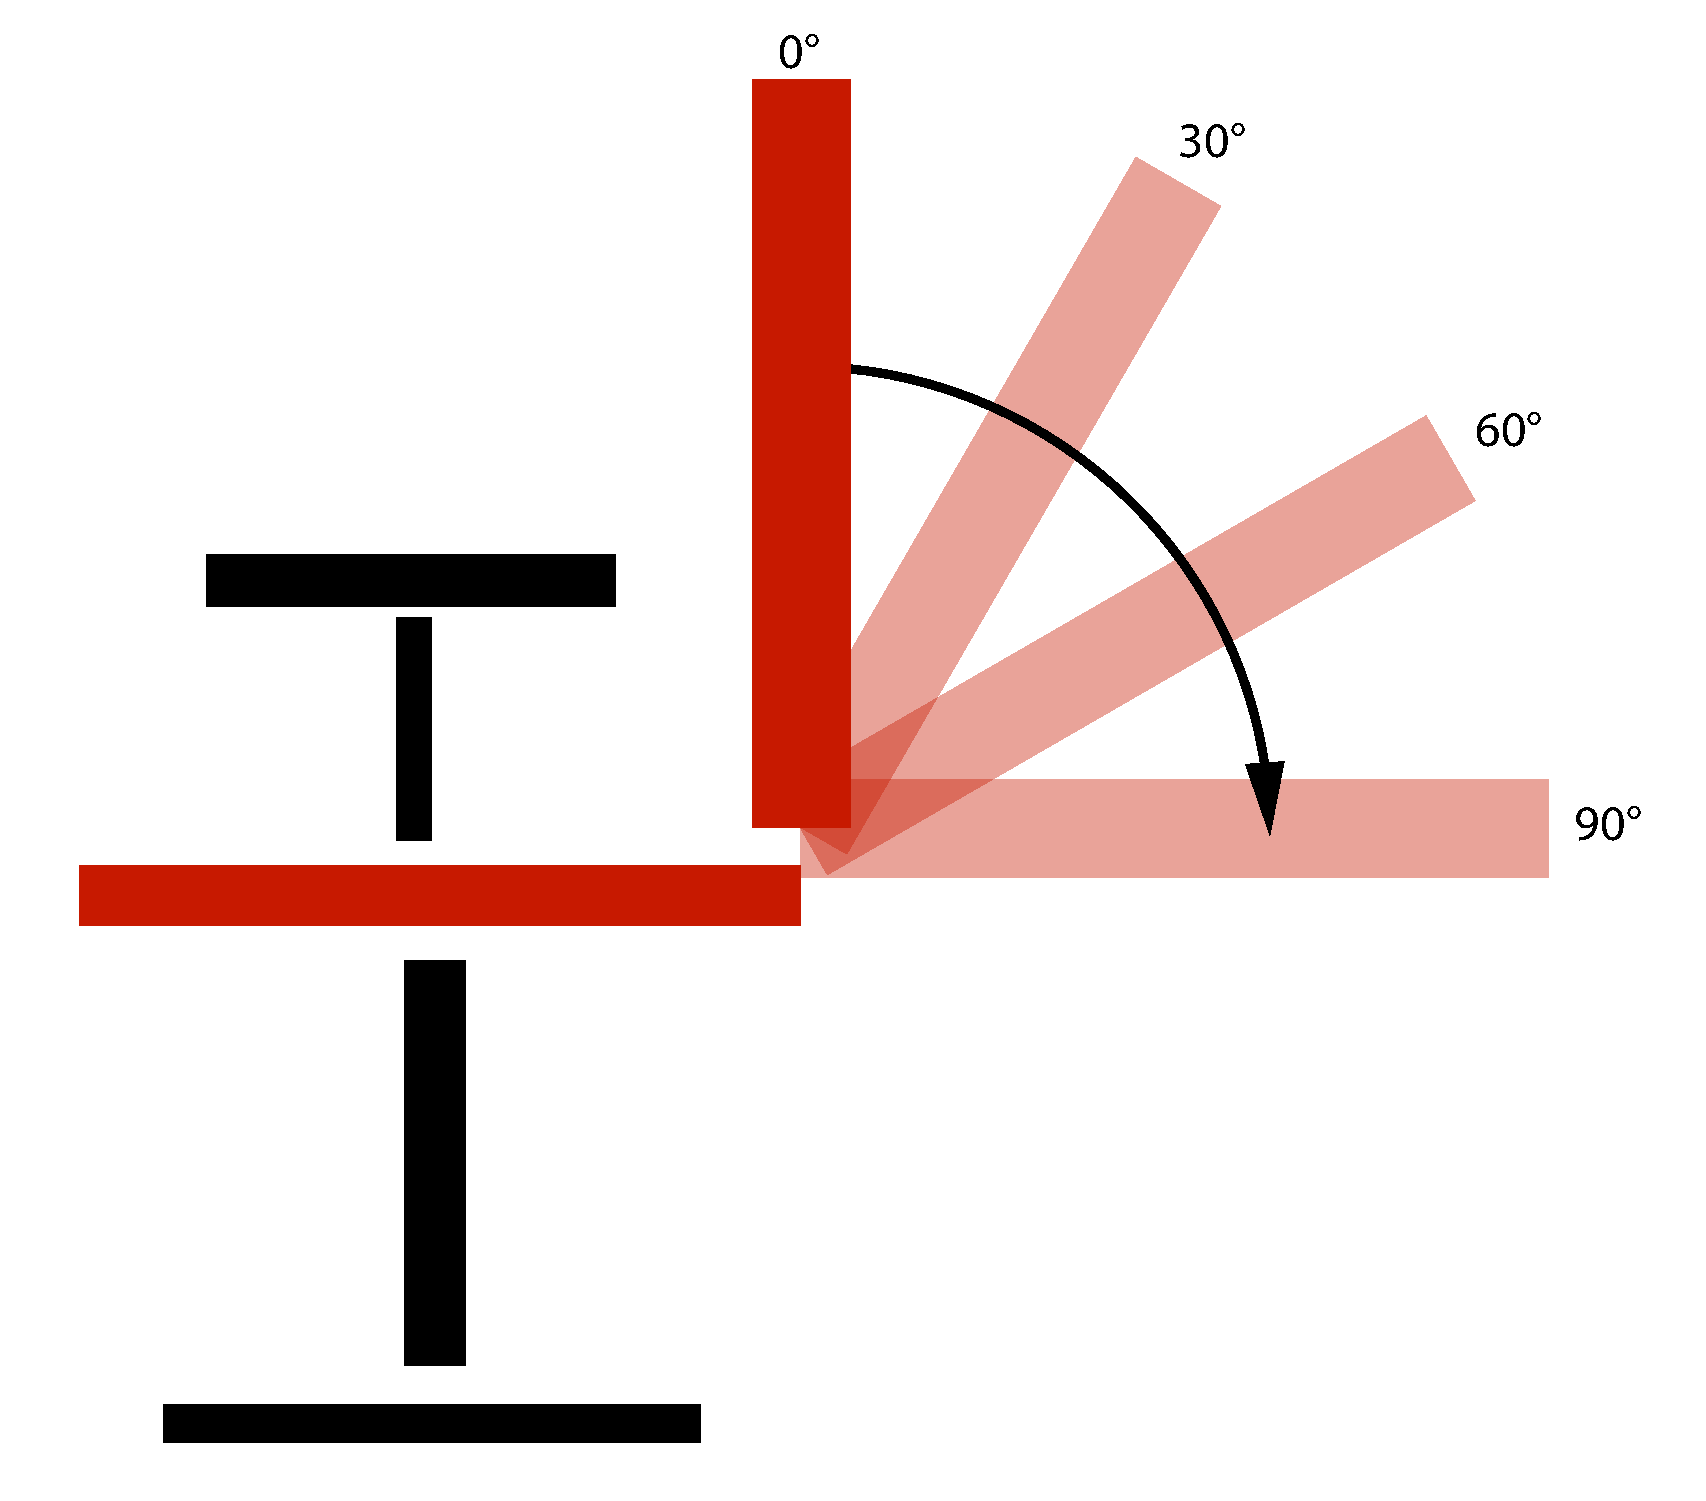
\includegraphics[width=0.8\textwidth]{./images/chair}
	\caption{Winkeleinstellungen vom verwendeten Stuhl in der Studie}
	\label{fig:counting}
\end{figure}
